\pdfoutput=1
\documentclass[11pt,a4paper]{article}

\usepackage[utf8]{inputenc}
\usepackage[T1]{fontenc}
\usepackage{lmodern}
\usepackage[a4paper,margin=2.5cm]{geometry}
\usepackage{amsmath,amssymb}
\usepackage{graphicx}
\usepackage{booktabs}
\usepackage{array}
\usepackage{tabularx}
\usepackage{microtype}
\usepackage[round,authoryear]{natbib}
\usepackage{xcolor}
\usepackage[most]{tcolorbox}
\usepackage{caption}
\usepackage{enumitem}
\usepackage{placeins}
\usepackage{url}
\usepackage{xurl}
\usepackage[hidelinks]{hyperref}
\usepackage[nameinlink,capitalise,noabbrev]{cleveref}

\definecolor{cbase}{HTML}{2A78D6}
\definecolor{ink2}{HTML}{52514E}
\definecolor{panel}{HTML}{F4F3EF}
\hypersetup{colorlinks=true,linkcolor=cbase!80!black,citecolor=cbase!80!black,urlcolor=cbase!80!black}

\captionsetup{font=small,labelfont=bf,labelsep=colon,skip=6pt}
\captionsetup[table]{position=top}
\setlist{itemsep=2pt,topsep=4pt}
\renewcommand{\arraystretch}{1.12}
\newcommand{\sourcenote}[1]{\par\vspace{3pt}{\footnotesize\color{ink2}#1\par}}

\title{\textbf{Road Transport Electrification in Finland}\\[4pt]
\large Electricity Consumption Scenarios to 2050 and Power-Market Implications}
\author{Juhani Merilehto\thanks{ORCID 0000-0002-8010-3725. The analysis and views expressed are solely those of the author and do not represent any employer or affiliated institution.}}
\date{November 2026}

\begin{document}
\maketitle
\vspace{-1.2em}
\begin{center}\small\color{ink2}Copyright \textcopyright{} 2026 Juhani Merilehto. Text, figures and data are licensed under CC BY 4.0.\end{center}

\begin{abstract}
\noindent An earlier study concluded that road-transport electrification in Finland is a secondary national energy-volume driver but a first-order distribution-network and flexibility issue, with 2.24--3.82~TWh of consumption in 2030 \citep{merilehto2026road2030}. This paper tests whether that conclusion still holds in 2050, when most cars, vans, buses and many trucks are electric. The 2030 low, base and high states are reproduced from their published inputs and retained exactly. A cohort stock-flow model by vehicle segment, calibrated to the 2025 Statistics Finland value of 1,112~GWh and to the observed electric vehicle stocks, then carries them to 2050.

Road-transport electricity reaches 3.5--7.1~TWh in 2035 and 8.2--14.9~TWh in 2050 (Base 5.4 and 12.0~TWh). That is 4.5--11\% of the 134--180~TWh of final electricity consumption in the 2050 scenarios of Finland's Long-term Climate Plan, so road transport remains secondary against the national total. It also remains well below data centres once their buildout is taken from project capacities: about 4.5~GW under construction and over 11~GW announced correspond to roughly 25--62~TWh a year, against which 2050 road transport is 13--59\%. The plan's own data-centre assumption of just over 10~TWh in three of its four 2050 scenarios is below what is already being built. Average load in 2050 is 0.9--1.7~GW. An illustrative winter-evening charging block of 6.3--11.2~GW, equal to 40--72\% of the January 2026 consumption record, compares with an overnight managed block of 2.9--5.2~GW. A synchronised restart after curtailment can exceed the evening block. Heavy vehicles add 13--20\% of the energy but a distinct depot and corridor connection problem. The scenarios are assumed planning states, not forecasts.
\end{abstract}

\begin{tcolorbox}[enhanced,colback=panel,colframe=panel,arc=2pt,boxrule=0pt,left=8pt,right=8pt,top=6pt,bottom=6pt,
  title={\textbf{Key findings}},coltitle=black,fonttitle=\small,attach title to upper={\par\vspace{2pt}}]
\small
\begin{itemize}[leftmargin=12pt]
  \item \textbf{Against the national total, the core conclusion holds in 2050.} Road transport reaches 8.2--14.9~TWh, 4.5--11\% of the national final electricity consumption in the Long-term Climate Plan's 2050 scenarios (Base 7--9\%).
  \item \textbf{Against data centres, it also holds, if their buildout is taken from project capacities.} About 4.5~GW of data centres are under construction and over 11~GW announced, roughly 25--62~TWh a year at Fingrid's implied utilisation; the author's base estimate for 2035 is over 30~TWh. The whole electrified road fleet of 2050 (8.2--14.9~TWh) is 13--59\% of that range. The plan's assumption of just over 10~TWh in three of its four 2050 scenarios would make the two comparable, but it is below what is already being built.
  \item \textbf{Timing still decides the power footprint.} In 2050 an illustrative concentrated winter-evening block of 6.3--11.2~GW compares with a managed overnight block of 2.9--5.2~GW; the two blocks differ by 3.4--5.9~GW but occur at different hours.
  \item \textbf{Rebound is a design constraint.} After a four-hour curtailment, a synchronised restart with well-equipped home chargers lifts Base light-duty charging to 13~GW. With weaker charging equipment, full recovery takes 7--10 hours and no longer fits within a ten-hour night window.
  \item \textbf{Heavy vehicles are a connection problem, not a volume problem.} They use 13--20\% of the 2050 energy, but a 100-bus depot draws 2.4~MW with spread charging and 13.5~MW if all chargers start on return. National corridor charging peaks at 75--354~MW, equivalent to 60--300 megawatt chargers at full power.
  \item \textbf{The retained 2030 states have moved relative to the data.} At the end of September 2026 the battery-electric car stock already matched the model's end-2026 Low level, and subtracting 2025 rail use from Fingrid's 2030 transport outlook gives an illustrative road equivalent above the High state. The retained Low state now describes a stall.
\end{itemize}
\end{tcolorbox}

%=====================================================================
\section{Introduction}
%=====================================================================
Electricity used in Finnish road transport crossed 1~TWh for the first time in 2025. Statistics Finland reports 1,112~GWh, up 43\% on 2024 \citep{statfin2026release,statfin2026_12sz}. An earlier study from June 2026 \citep{merilehto2026road2030} extrapolated that series to 2030 and reached a central conclusion: road-transport electrification is a secondary national energy-volume driver compared with data centres, industrial electrification and hydrogen, but a first-order distribution-network and flexibility issue, because charging is mass-distributed, time-shiftable and tariff-sensitive. Its base case reached about 3.0~TWh in 2030, within 2.24--3.82~TWh.

A 2030 horizon cannot test that conclusion where it matters. In 2030 most of the Finnish vehicle fleet still runs on liquid fuels. By 2050, under the EU's CO$_2$ rules for new vehicles, most cars, vans and urban buses and a large share of trucks would be electric. If road transport stays a secondary energy load even then, the conclusion is robust. If it becomes a primary one, the planning priorities change.

This paper keeps the core question and the 2030 states of the earlier study and extends them to 2050. It reproduces the 2030 study and reconciles its statistical boundary with Fingrid's outlook (\cref{sec:retained,sec:boundary}). It updates the evidence on fleet, policy, heavy-vehicle charging and flexibility to November 2026 (\cref{sec:evidence}). It replaces the CAGR extrapolation with a segment stock-flow model that reproduces the observed electric vehicle stocks, the 2025 statistic and the 2030 states exactly (\cref{sec:model}). It then reports annual energy, average load, illustrative charging blocks and heavy-vehicle depot and corridor loads to 2050, with robustness tests and a comparison against national scenarios (\cref{sec:results,sec:materiality,sec:robust}).

The scenarios are assumed planning states. They are conditional envelopes for grid and market planning, not forecasts with assigned probabilities.

%=====================================================================
\section{The 2030 study and what is retained}\label{sec:retained}
%=====================================================================
The 2030 study used Statistics Finland's PX-Web table 12sz, electricity in road transport, 2012--2025, as extracted on 12 June 2026 and deposited with the report \citep{merilehto2026road2030}. It measured growth with year-on-year rates, annual increments and compound annual growth rates (CAGR) over six windows. The series moved through emergence (2012--2017), take-off (2018--2021) and scaling (2022--2025), with percentage growth slowing to 43\% in 2025 while the annual increment reached a record 335~GWh.

The forward scenarios were a transparent CAGR extrapolation from the 2025 value, $E_{2030}=1{,}112\times(1+g)^5$, with $g=$ 15\%, 22\% and 28\% for the low, base and high cases (2,237, 3,005 and 3,821~GWh). A bottom-up check by segment (0.50 million BEVs at 14,000~km and 0.185~kWh/km, 0.22 million PHEVs, 0.08 million vans, 2,000 buses, 8,000 trucks and a residual) summed to 3.00~TWh. The study noted that a passenger-car reconstruction could not explain the official statistic, and that commercial segments, PHEV electric driving, charging losses, winter consumption and allocation all mattered. For power, it converted 3.0~TWh to an average 343~MW and showed that 70\% of daily charging in three evening hours would form a 1.9~GW block, against 0.8~GW if spread over ten off-peak hours. A flexibility table gave 300--1,250~MW of controllable charging power from 0.5 million BEVs.

All of these numbers are reproduced in code from the stated inputs (\cref{tab:reproduction} in the appendix), and the script stops if any differ. The archived 12sz CSV is used unchanged and verified by its checksum. A re-extraction on 8 November 2026 returns the same 2012--2025 values, although the table was updated on 1 July 2026 \citep{statfin2026_12sz}. The 2025 value is still preliminary.

What is retained: the core question, the statistical series and its boundary, the three 2030 values, and the charging-block framing. What changes: the 2030 values are now reached by a stock-flow path rather than a CAGR, and everything after 2030 is constructed from vehicle stocks, entries, mileage and intensity.

%=====================================================================
\section{Evidence update to November 2026}\label{sec:evidence}
%=====================================================================
\subsection{Fleet and registrations}
At the end of 2025 Finland had 2,696,432 passenger cars in traffic use, of which 164,705 were battery-electric (BEV) and 187,039 plug-in hybrid (PHEV); 332,711 vans (6,502 BEV); 88,569 lorries over 3.5~t (222 electric); and 11,173 buses (1,106 electric) \citep{statfin2026_11ie}. The total car stock fell in 2025 partly because 88,365 cars were removed in a register correction \citep{aut2026review}. In 2025 BEVs were 37.2\% of 71,888 new cars, 18.3\% of new vans, 3.1\% of new trucks and 35\% of 420 new buses; a further 41,092 used cars were imported \citep{aut2026review}.

Adoption has kept accelerating. By the third quarter of 2026 there were 209,694 BEV and 195,426 PHEV cars in traffic, together 14.6\% of the car fleet, and BEVs took 62.1\% of new-car registrations in September 2026 \citep{sahkoinenliikenne2026q3}. Electric vans numbered 7,820, electric trucks 279 (178 over 12~t) and electric buses 1,284. Public charging comprised 17,511 AC points and 5,612 DC points, 4,555 of them rated at 150~kW or more \citep{sahkoinenliikenne2026q3}.

Statistics Finland's traffic performance series gives 39.0 billion vehicle-km for cars, 5.5 billion for vans, 3.0 billion for lorries and 566 million for buses in 2025 \citep{statfin2026traffic,statfin2026_12jx}. Divided by the stock in traffic, that is 14,470~km per car, 16,410 per van, 33,840 per lorry and 50,660 per bus.

\subsection{Policy}
EU law still requires a 100\% CO$_2$ reduction for new cars and vans from 2035 against 2021, after 55\% (cars) and 50\% (vans) in 2030 \citep{eprs2026co2}. In December 2025 the Commission proposed 90\% for 2035, with credits of up to 3 percentage points for renewable fuels and 7 for EU-made low-carbon steel, and 40\% for vans in 2030 \citep{eprs2026co2}. On 4 November 2026 the Parliament's environment committee adopted its position by 48 votes to 30 with 2 abstentions: a 2035 car target that falls to an effective 87.5\% when the maximum 7.5 percentage points of low-carbon-steel credits are used, and, for vans, 35\% in 2030 and 80\% in 2035 \citep{eunews2026envi,electrive2026envi}. The plenary vote is expected in December 2026, after which Parliament negotiates with the Council, which has not adopted its position \citep{electrive2026envi}. Current law is therefore unchanged. In this paper the rules enter only through the electric-share ceilings, which are model assumptions (\cref{sec:states}).

For heavy-duty vehicles, Regulation (EU) 2024/1610 sets fleet CO$_2$ reductions of 15\% for 2025--2029, 45\% for 2030--2034, 65\% for 2035--2039 and 90\% from 2040, and requires 90\% of new urban buses to be zero-emission in 2030 and 100\% in 2035; inter-urban buses are exempt and the regulation is reviewed in 2027 \citep{oeil2024hdv}.

Finland's 2021 roadmap for fossil-free transport aims to halve domestic transport emissions by 2030 from 2005 and to reach zero-emission transport by 2045, and assumed about 700,000 electric cars and 45,000 electric vans in 2030 \citep{vn2021roadmap}. Under the EU effort-sharing regulation Finland must cut non-ETS emissions by 50\% by 2030, and the national climate target is carbon neutrality in 2035 \citep{traficom2025tilli}. The Long-term Climate Plan of February 2026 sets out four scenarios to 2050 in which electricity use in transport rises to 11--15~TWh \citep{meae2026ltcp}. The fuel distribution obligation was lowered to 13.5\% for 2023 and 2024 \citep{energiavirasto2026jakelu}, rose to 19.5\% in 2026 and is legislated at 22.5\% for 2027 and 31\% for 2028 \citep{skal2026}; the 2030 level is 34\% \citep{ieaamf2025finland}. EU emissions trading for road fuels starts in 2028, a year later than first decided \citep{skal2026}. The national purchase subsidy for heavy electric vehicles ended at the end of 2024 \citep{traficom2025tilli}. A high renewable-diesel obligation lowers the carbon advantage of electric trucks, which is one reason the heavy-duty states below are wider than the light-duty ones.

\subsection{Megawatt charging and heavy-vehicle infrastructure}
Finland's first public megawatt charging system (MCS) station opened for trucks at Mussalo, Kotka, in December 2025, with 1,800~kW from three 600-kW units feeding one MCS outlet of up to 1.2~MW and four CCS outlets of up to 560~kW \citep{kempower2026kotka}. The first public MCS session in Finland was reported in October 2026 \citep{electrive2026plugit}. The EU's Alternative Fuels Infrastructure Regulation requires heavy-duty charging pools every 60~km on the core TEN-T network and every 100~km on the comprehensive network by the end of 2030, with at least 3,600~kW per pool on the core network, 1,500~kW on the comprehensive network and 1,800~kW at urban nodes \citep{icct2023afir}.

Most truck energy can come from depots. In France, Germany and the United Kingdom 40--50\% of trucks drive less than 200--300~km a day; a depot of 40 trucks needs about 2~MW of connection at 50~kW per truck or 6~MW at 150~kW \citep{te2025depot}. Real-world data from German rigid electric trucks show an average of 0.96~kWh/km, rising with gross weight \citep{oeko2025elv}.

\subsection{Flexibility, smart charging and distribution networks}
Fingrid expects demand-side response to grow significantly but does not quantify it, and it notes that not all new electrification load can flex \citep{fingrid2026prospects,fingrid2026q3}. Battery storage reached about 1.6~GW by summer 2026 \citep{fingrid2026prospects}. Data centres drive the growth. Announced Finnish data-centre projects sum to more than 11~GW of nominal capacity at their maximum, of which about 4.5~GW is under construction; signed data-centre connection agreements rose from about 3~GW to nearly 5~GW between June and August 2026 and kept growing in August--September, which is why the author regards the lower end of Fingrid's 2035 consumption range as cautious \citep{merilehto2026blog}. The author's market assessment adds that data centres are unlikely to offer much flexibility because of their high profitability, so it must increasingly come from other market actors: electric boilers (over 3~GW nominal, but at most about 1.1~GW in any hour so far), batteries, and households, of which only a third hold spot-price contracts \citep{merilehto2026blog}.

Electric vehicles were the most-tested flexibility source across 45 Nordic demand-side initiatives \citep{norden2025flex}. In a Finnish distribution pilot with 150 EV drivers, chargers responded to down-regulation in about a minute, and the Energy Authority lets network companies use up to 1\% of revenue on flexibility in 2024--2027 \citep{kemp2026enlit}. Distribution-level studies find that uncontrolled charging raises reinforcement needs and that price-based charging can itself create regional peaks when many chargers respond to the same signal \citep{lut2026charging,borenius2022scenarios}. Controlled charging under peak-power-based tariffs reduces residential peaks \citep{simolin2020}, and the IEA identifies tariffs, connection rules and flexibility remuneration as the main levers \citep{iea2022grid}.

Bidirectional charging is still at pilot scale. A Swedish pilot is installing about 200 V2G chargers in SE3 and SE4, running to 2028 \citep{vattenfall2026v2g}. Industry assessments cite the scarcity of V2G-enabled vehicles and chargers as the main barrier \citep{ey2025flex}. EV charging networks already sell FCR-D reserve in the Nordics, where the minimum Finnish bid is 1~MW \citep{virta2026fcrd}. Fingrid's 2040 vision varies the assumption: in its data-centre-led scenario only a small share of EV charging responds to price, whereas in two other scenarios price-steered and bidirectional charging is widespread \citep{fingrid2025vision}.

%=====================================================================
\section{System boundaries: road transport and ``transport'' elsewhere}\label{sec:boundary}
%=====================================================================
The 12sz series used here covers road transport only. Fingrid's Q3/2026 outlook describes transport electricity rising ``from the current level of approximately two terawatt-hours to around 5 terawatt-hours by 2030 and around 8 terawatt-hours by 2035'' \citep{fingrid2026prospects}. The gap with 1.1~TWh in 2025 is mainly a boundary difference, and it should be explained before comparing projections.

\begin{table}[t]
\centering
\caption{Road transport in Statistics Finland 12sz and ``transport'' in Fingrid's and the ministry's publications (TWh).}
\label{tab:boundary}
\footnotesize
\setlength{\tabcolsep}{4.5pt}
\begin{tabular}{@{}lrrrrrr@{}}
\toprule
 & 2024 & 2025 & 2030 & 2035 & 2040 & 2050 \\
\midrule
Statistics Finland, road transport & 0.78 & 1.11 & -- & -- & -- & -- \\
Statistics Finland, rail transport & 0.69 & 0.66 & -- & -- & -- & -- \\
Statistics Finland, all transport & 1.47 & 1.78 & -- & -- & -- & -- \\
\addlinespace
Fingrid Q3/2026 outlook, ``transport'' & & $\approx$2 & $\approx$5 & $\approx$8 & & \\
Fingrid vision 2040, ``transport'' & 1 & & & & 10 & \\
Long-term Climate Plan, transport & & & & & & 11--15 \\
\addlinespace
Fingrid less 2025 rail (illustrative road equivalent) & & 1.3 & 4.3 & 7.3 & 9.3 & \\
This paper, road, Low--High & & 1.11 & 2.24--3.82 & 3.54--7.11 & 5.14--10.28 & 8.16--14.86 \\
\bottomrule
\end{tabular}
\sourcenote{Statistics Finland 12sz \citep{statfin2026_12sz}; domestic navigation and air use no electricity in 12sz, so all transport electricity is road plus rail. Fingrid \citep{fingrid2026prospects,fingrid2025vision}; Fingrid does not define the category, and its outlook counts electricity for transport e-fuels under industry. Ministry of Economic Affairs and Employment \citep{meae2026ltcp}. The road-equivalent row subtracts 2025 rail electricity only, as an illustration.}
\end{table}

Three points follow from \cref{tab:boundary}. First, Statistics Finland's total transport electricity in 2025 is 1.78~TWh, of which rail is 0.66~TWh. That is consistent with Fingrid's ``approximately two'' TWh, so Fingrid's current figure most plausibly covers road and rail together. Second, Fingrid's earlier 2040 vision gives 1~TWh for 2024; because road (0.78~TWh) and all transport (1.47~TWh) both round to about 1~TWh, that figure does not show which boundary was used. Third, if 2025 rail use is subtracted, Fingrid's 2030 figure gives an illustrative road equivalent of about 4.3~TWh, above the retained High state; the same subtraction gives about 7.3~TWh in 2035, just above the High state, and about 9.3~TWh in 2040, between Base and High. The ministry's 11--15~TWh for all transport in 2050 compares with 8.8--15.5~TWh for road in this paper plus 2025 rail electricity. Fingrid's outlook therefore embeds faster near-term growth than the 2030 study but converges on similar magnitudes by the mid-2030s, and the ministry's 2050 range brackets the Base state. Any residual difference can come from distribution losses on the grid side, other transport uses such as shore power, or different adoption assumptions; the sources do not allow these to be separated.

%=====================================================================
\section{Method}\label{sec:model}
%=====================================================================
\subsection{Stock-flow structure}
The model follows six segments: battery-electric cars, plug-in hybrid cars (electric driving only), vans, regional trucks, long-haul trucks and buses. For each segment $c$, the fleet $S_c$ is held at its 2025 level (varied in the robustness tests). Annual fleet entries, new registrations plus used imports where reported, are $A_c=S_c/\bar L_c$, where the mean register life $\bar L_c$ is set so that the 2025 entries are consistent with a steady fleet. For cars, 112,980 entries a year imply $\bar L=23.9$ years, close to the 23.0-year average scrapping age reported for 2025 \citep{aut2026review}. Electric entries are $A_c z_c(t)$, where $z_c$ is the electric share of entries. Each annual cohort survives along a Weibull curve $s_c(a)$ with shape 3 and mean $\bar L_c$.

Historical electric cohorts are backed out of the observed year-end stocks \citep{statfin2026_11ie}, so that survivors are not double-counted. With cohorts entering mid-year,
\begin{equation}\label{eq:cohorts}
N_{c,v}=\frac{O_{c,v}-\sum_{w<v}N_{c,w}\,s_c(v-w+0.5)}{s_c(0.5)},\qquad v=2012,\dots,2025,
\end{equation}
where $O_{c,v}$ is the observed electric stock at the end of year $v$. The surviving cohorts reproduce every observed year-end stock from 2012 to 2025 exactly, except where the registered stock fell below the survivors of earlier cohorts (electric buses in 2018), and they reproduce the 2025 stock of every segment exactly. The script asserts both (\texttt{data/stock\_check.csv}).

Electricity in year $t$ is
\begin{equation}\label{eq:energy}
E(t)=\kappa\,u(t)\sum_{c\in\mathrm{LD}}\sum_{v\le t}N_{c,v}\,s_c(t-v)\,k_c(t-v)\,e_c(1+\lambda)\;+\;\sum_{c\in\mathrm{HD}}\sum_{v\le t}N_{c,v}\,s_c(t-v)\,k_c(t-v)\,e_c(1+\lambda),
\end{equation}
where $k_c(a)$ is annual mileage at age $a$, $e_c$ is energy intensity at the vehicle and $\lambda=10\%$ is the charging loss; a cohort counts for half a year in its entry year. LD denotes light duty (cars, PHEV electric driving, vans) and HD heavy duty. Mileage declines with age, $k_c(a)=k_{c,0}\,e^{-a/\theta_c}$. The constant $k_{c,0}$ is set so that the steady-state fleet average equals the 2025 average from \citet{statfin2026_12jx}, and $\theta_c$ so that a new vehicle drives a stated multiple of the average: 1.4 for cars (about 20,300~km), 1.5 for vans and buses, 1.8 for regional and 2.2 for long-haul trucks. Lorries are split 60:40 into regional and long-haul segments; regional trucks average 22,000~km and long-haul trucks about 51,600~km, which reproduces the 2025 lorry vehicle-km. All 2025 electric lorries are assigned to the regional segment.

Intensities are 0.185~kWh/km for BEV cars and 0.19~kWh/km over 6,000 electric km for PHEVs, 0.25 for vans and 1.0 for buses (all retained from the 2030 study), 1.0 for regional trucks \citep{oeko2025elv} and 1.3 for long-haul trucks (assumption, including a cold-climate margin). The 10\% charging loss lies between ADAC's measured 5--7\% at an 11-kW wallbox and 13--24\% at a household socket \citep{popa2026adac}.

\subsection{Calibration to the official statistic}
With these engineering values the 2025 cohorts would use 0.87~TWh in light duty and 0.09~TWh in heavy duty, against an official 1,112~GWh. The light-duty factor $\kappa=1.17$ closes the gap. It stands for what the engineering reconstruction misses: winter consumption, above-average use of young electric cars beyond the mileage profile, losses above 10\%, and the allocation method of the statistic, which is not published. Heavy duty is not scaled because it is too small in 2025 to be informative. The age-mileage profile explains most of the gap that the 2030 study left as a residual; without it $\kappa$ would be about 1.6. $\kappa$ is held constant in the reported states and tested in \cref{sec:robust}.

\subsection{Assumed planning states}\label{sec:states}
The electric share of entries starts from its observed 2025 value: 41\% BEV and 18\% PHEV for cars (new cars plus used imports), 20\% for vans, 3.3\% for lorries and 35\% for buses. For light duty, the share changes linearly to 2030 by $\delta$ percentage points a year (0 in Low, +5 in Base, +10 in High). After 2030 it follows a logistic curve rescaled to start exactly at the 2030 value:
\begin{equation}\label{eq:logistic}
z_c(t)=z_{c,2030}+\bigl(z_c^{\max}-z_{c,2030}\bigr)\,\frac{\sigma\!\left(\frac{t-t_c}{w_c}\right)-\sigma\!\left(\frac{2030-t_c}{w_c}\right)}{1-\sigma\!\left(\frac{2030-t_c}{w_c}\right)},\qquad \sigma(x)=\frac{1}{1+e^{-x}},
\end{equation}
with ceiling $z_c^{\max}$, midpoint $t_c$ and width $w_c$. The rescaling makes the path continuous and monotone: in Base the BEV share of car entries is 66.2\% in 2030, 71.0\% in 2031 and 75.5\% in 2032. Heavy-duty segments use the same form from their observed 2025 share. PHEV entries stay at the 2025 share to 2030 and decline linearly to the 2040 value in \cref{tab:states}. The combined BEV and PHEV share of car entries is capped at 100\% in every state and sensitivity: BEVs have priority and PHEVs receive at most the remainder, which the script asserts each year. The cap binds only in High, where the PHEV share falls from 18\% in 2029 to 8.8\% in 2030, 1.6\% in 2035 and zero from 2040, so that plug-in vehicles take all car entries from 2030 (\texttt{data/car\_entry\_shares.csv}). A genuine delay of $d$ years holds $z_{c,2030}$ for $d$ years and then evaluates \cref{eq:logistic} at $t-d$, without renormalising to the 2050 value.

\begin{table}[t]
\centering
\caption{Assumed planning states: electric share of fleet entries (ceiling $z^{\max}$, midpoint $t_c$).}
\label{tab:states}
\small
\begin{tabular}{@{}lccc@{}}
\toprule
Segment & Low & Base & High \\
\midrule
Cars, BEV, 2026--2030 change $\delta$ (pp/yr) & 0 & +5 & +10 \\
Cars, BEV, after 2030 & 85\%, 2033 & 95\%, 2030 & 100\%, 2028 \\
Cars, PHEV share of entries in 2040 & 8\% & 2\% & 0\% \\
Vans, 2026--2030 change $\delta$ (pp/yr) & 0 & +5 & +10 \\
Vans, after 2030 & 80\%, 2034 & 95\%, 2031 & 100\%, 2029 \\
Regional trucks & 55\%, 2040 & 85\%, 2036 & 95\%, 2033 \\
Long-haul trucks & 35\%, 2044 & 70\%, 2039 & 90\%, 2036 \\
Buses (urban and coach) & 65\%, 2030 & 80\%, 2028 & 95\%, 2027 \\
\addlinespace
\emph{Solved:} light-duty electricity per EV in 2030, $u$ (2025 = 1) & 0.94 & 1.09 & 1.21 \\
\bottomrule
\end{tabular}
\sourcenote{Widths $w_c$ 2.5--4 years. Fleet sizes, lives, mileage and intensities are common to all states. $u$ is solved by bisection so that each state reproduces its retained 2030 value exactly; it ramps linearly over 2026--2030 and is then held.}
\end{table}

The ceilings are model assumptions informed by the EU rules: 85--100\% of car entries electric, allowing for the proposed 87.5--90\% targets and for used imports from countries with older fleets; urban buses near 100\% but coaches exempt; and long-haul trucks well below the EU fleet target in Low and Base because Finnish long-haul is cold, long-distance and served by a rising renewable-diesel obligation.

One parameter per state is solved: $u$, light-duty electricity per EV in 2030 relative to 2025. It makes each state reproduce its retained 2030 value exactly (to 0.5~MWh), and the script asserts this together with the 2025 value. $u$ also reads as a diagnostic. Base needs 9\% more electricity per light-duty EV by 2030 than in 2025 and High 21\%, matching the 2030 study's description of High as having higher average EV utilisation. Low needs 6\% less and electric entry shares frozen at their 2025 level. With entry shares frozen and $u=1$, 2030 would reach 2.35~TWh, already above the Low state.

\subsection{Charging blocks}
Annual energy is converted to average load over 8,760 hours. Charging is then shown as illustrative blocks on a winter day, extending the 2030 study's framing. Winter-day energy is 25\% above the annual mean for light duty and buses and 15\% for trucks (assumption, informed by a measured 2.4~kWh/100~km increase per 5~°C below 10~°C; \citealp{xu2019seasonal}). The \emph{evening block} combines light-duty charging concentrated in the evening (70\% of daily energy in three hours, or 50\% in four in the moderate case), depot charging started on return (60\% of buses' and regional trucks' energy and half of long-haul energy in four hours) and corridor charging at its average daytime level. The \emph{night block} spreads light-duty energy over ten night hours and depot energy over eight; corridor charging is assumed to take place over 14 daytime hours, with a peak hour 1.4 times its average, and is not included at night. The two blocks occur at different hours. Their difference is reported as such; it is not a modelled reduction of the national peak, and the model does not estimate adequacy.

%=====================================================================
\section{Results}\label{sec:results}
%=====================================================================
\subsection{Annual electricity to 2050}
\Cref{fig:paths} and \cref{tab:checkpoints} show the paths. From the retained 2030 values, road-transport electricity reaches 3.5--7.1~TWh in 2035, 5.1--10.3~TWh in 2040 and 8.2--14.9~TWh in 2050. The Base state reaches 5.4~TWh in 2035 and 12.0~TWh in 2050, when 2.09 million battery-electric cars, 77\% of today's car fleet, are in traffic. Growth slows after 2040 in every state, as fleet turnover rather than the electric share of new vehicles becomes the limiting step.

\begin{figure}[t]
\centering
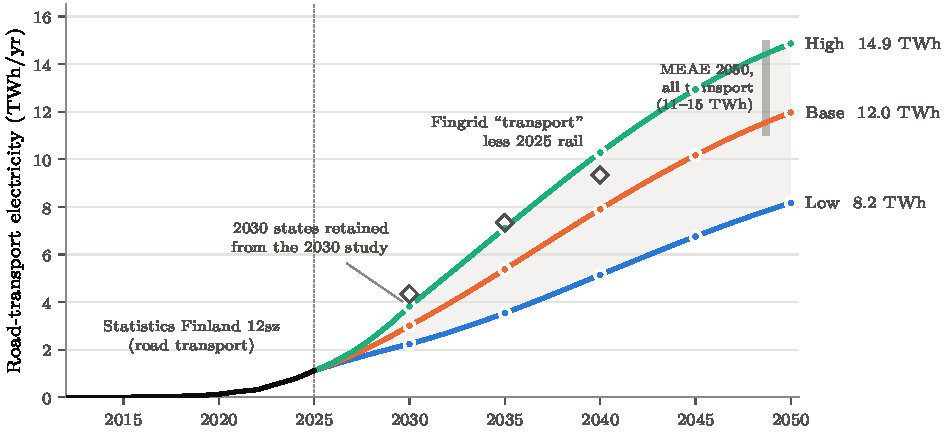
\includegraphics[width=\linewidth]{figures/fig1_paths.pdf}
\caption{Road-transport electricity, 2012--2050, linear scale. Black: Statistics Finland 12sz. Coloured: assumed planning states, with the 2030 values retained from the earlier study and checkpoints marked. Diamonds: Fingrid's ``transport'' less 2025 rail electricity. Grey bar: electricity in all transport in 2050 in the Long-term Climate Plan (\cref{tab:boundary}).}
\label{fig:paths}
\end{figure}

\begin{table}[t]
\centering
\caption{Checkpoint results by state.}
\label{tab:checkpoints}
\small
\begin{tabular}{@{}lrrrrrr@{}}
\toprule
State & 2025 & 2030 & 2035 & 2040 & 2045 & 2050 \\
\midrule
\multicolumn{7}{@{}l}{\emph{Annual electricity (TWh)}} \\
Low & 1.11 & 2.24 & 3.54 & 5.14 & 6.76 & 8.16 \\
Base & 1.11 & 3.01 & 5.38 & 7.90 & 10.17 & 11.96 \\
High & 1.11 & 3.82 & 7.11 & 10.28 & 12.93 & 14.86 \\
\multicolumn{7}{@{}l}{\emph{Annual average load (MW)}} \\
Low & 127 & 255 & 404 & 587 & 772 & 932 \\
Base & 127 & 343 & 614 & 902 & 1,161 & 1,366 \\
High & 127 & 436 & 811 & 1,173 & 1,476 & 1,697 \\
\multicolumn{7}{@{}l}{\emph{Battery-electric cars in traffic, year end (thousand)}} \\
Low & 165 & 394 & 680 & 1,041 & 1,401 & 1,708 \\
Base & 165 & 478 & 905 & 1,361 & 1,768 & 2,089 \\
High & 165 & 563 & 1,086 & 1,582 & 2,001 & 2,314 \\
\multicolumn{7}{@{}l}{\emph{Heavy-duty share of road-transport electricity (\%)}} \\
Low & 8 & 7 & 8 & 9 & 11 & 13 \\
Base & 8 & 7 & 8 & 11 & 15 & 17 \\
High & 8 & 6 & 9 & 14 & 17 & 19 \\
\bottomrule
\end{tabular}

\sourcenote{2025 equals the Statistics Finland value; 2030 equals the retained 2030 states. Full annual paths: \texttt{data/paths.csv}.}
\end{table}

Cars dominate throughout (\cref{fig:segments}). In 2050 battery-electric cars use 5.9--10.2~TWh. Heavy duty rises from 6--7\% of the total in 2030 to 13--20\% in 2050, and long-haul trucks are the fastest-growing segment after 2035. The heavy-duty share is the least certain part of the result because truck turnover is slow and the Finnish long-haul ceiling is an assumption.

\begin{figure}[t]
\centering
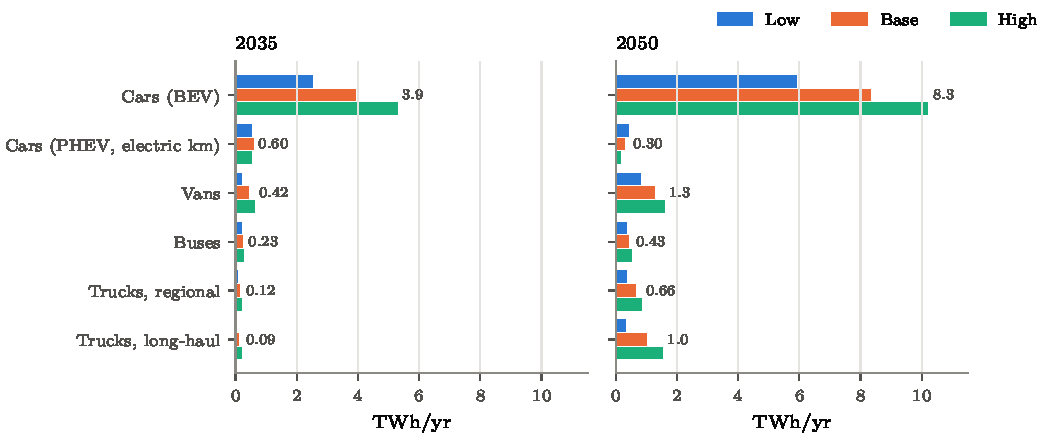
\includegraphics[width=\linewidth]{figures/fig2_segments.pdf}
\caption{Road-transport electricity by segment in 2035 and 2050. Numbers are Base values.}
\label{fig:segments}
\end{figure}

\subsection{Average load and charging blocks}
Energy and power diverge as the fleet electrifies (\cref{fig:peaks}, \cref{tab:loads}). In 2050 the average load is 0.9--1.7~GW. The concentrated evening block is 6.3--11.2~GW, about 6.6 times the average in Base; the moderate evening block is 3.6--6.8~GW. The night block of managed charging is 2.9--5.2~GW. The difference between the concentrated evening block and the night block grows from 1.0--1.7~GW in 2030 to 1.5--3.0~GW in 2035 and 3.4--5.9~GW in 2050. The blocks describe charging levels in different hours, so their difference is neither an amount of load moved between hours nor a change in the national peak.

\begin{figure}[t]
\centering
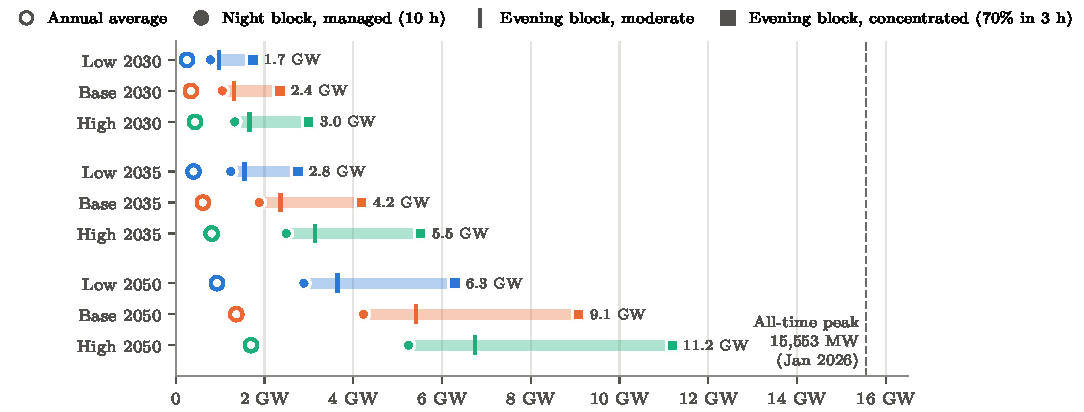
\includegraphics[width=\linewidth]{figures/fig3_peaks.pdf}
\caption{Annual average load and illustrative winter charging blocks by state and year. The bar spans the managed night block to the concentrated evening block, which occur at different hours. Dashed line: all-time Finnish consumption record.}
\label{fig:peaks}
\end{figure}

\begin{table}[t]
\centering
\caption{Average load and illustrative winter charging blocks (MW).}
\label{tab:loads}
\small
\begin{tabular}{@{}llrrrrrr@{}}
\toprule
Year & State & Average & Night block & Evening block, & Evening block, & Difference & Concentrated \\
 & & load & (managed) & moderate & concentrated & of blocks & / record \\
\midrule
2030 & Low & 255 & 784 & 977 & 1,745 & 961 & 11\% \\
 & Base & 343 & 1,050 & 1,310 & 2,352 & 1,303 & 15\% \\
 & High & 436 & 1,333 & 1,666 & 2,993 & 1,661 & 19\% \\
\addlinespace
2035 & Low & 404 & 1,242 & 1,549 & 2,759 & 1,516 & 18\% \\
 & Base & 614 & 1,884 & 2,359 & 4,192 & 2,308 & 27\% \\
 & High & 811 & 2,492 & 3,133 & 5,523 & 3,031 & 36\% \\
\addlinespace
2050 & Low & 932 & 2,890 & 3,643 & 6,292 & 3,402 & 40\% \\
 & Base & 1,366 & 4,233 & 5,413 & 9,077 & 4,844 & 58\% \\
 & High & 1,697 & 5,245 & 6,752 & 11,192 & 5,947 & 72\% \\
\bottomrule
\end{tabular}

\sourcenote{Night block: light-duty energy over 10 night hours and depot energy over 8 hours; no corridor charging. Evening blocks: light-duty charging (moderate: 50\% of daily energy in 4 hours; concentrated: 70\% in 3 hours), depots charging on return, corridor charging at its daytime average. Difference of blocks: concentrated evening minus night; the blocks occur at different hours. Record: 15,553~MW, January 2026 \citep{fingrid2026q1}.}
\end{table}

These blocks are not additions to the national peak in a strict sense. The concentrated case assumes that most of the light-duty fleet charges every winter evening at the same time, which overstates diversity-adjusted demand, and no hourly system profile is modelled. The value of the block is as a bound on what unmanaged, price-insensitive charging could add to evening load if tariffs and automation lag the fleet, which is the risk the 2030 study identified. That bound grows from 15\% of the 2026 record in the 2030 Base state to 58\% in 2050.

\subsection{Heavy vehicles: depots and corridors}
Heavy-duty charging is concentrated at fewer and larger sites (\cref{tab:heavy,tab:sites}). In the 2050 Base state about 7,200 electric buses and 30,000 electric trucks draw 0.85~GW from depots if charging is spread over eight hours and 1.0~GW if it starts on return. At site level the difference is larger. A 100-bus depot draws 2.4~MW if each bus's winter-day energy is spread over eight hours, but 13.5~MW if 150-kW chargers all start when the buses return. A 40-truck depot needs 2--6~MW depending on charger power \citep{te2025depot}.

\begin{table}[t]
\centering
\caption{Heavy-vehicle charging loads by state.}
\label{tab:heavy}
\footnotesize
\begin{tabular}{@{}llrrrrrr@{}}
\toprule
Year & State & E-buses & E-trucks & Depot, & Depot, & Corridor & MCS-point \\
 & & & (reg.\ / long-haul) & managed (MW) & on return (MW) & peak (MW) & at full power \\
\midrule
2035 & Low & 3,020 & 1,870 / 130 & 126 & 151 & 4 & 3 \\
 & Base & 3,490 & 3,490 / 700 & 192 & 230 & 20 & 16 \\
 & High & 4,060 & 5,690 / 1,620 & 286 & 343 & 46 & 38 \\
\addlinespace
2050 & Low & 5,910 & 11,110 / 2,830 & 445 & 534 & 75 & 62 \\
 & Base & 7,180 & 21,180 / 9,060 & 850 & 1,021 & 229 & 191 \\
 & High & 8,570 & 27,590 / 14,490 & 1,147 & 1,376 & 354 & 295 \\
\bottomrule
\end{tabular}

\sourcenote{Corridor: half of long-haul energy charged en route over 14 daytime hours; peak hour 1.4 times the average. The last column divides the national corridor peak by 1.2~MW: simultaneous chargers operating at full power, not a count of chargers or sites.}
\end{table}

\begin{table}[t]
\centering
\caption{Representative heavy-vehicle charging sites.}
\label{tab:sites}
\small
\begin{tabular}{@{}lr@{}}
\toprule
Site configuration & MW \\
\midrule
Bus depot, 100 e-buses, 150 kW chargers, all start on return (simultaneity 0.9) & 13.5 \\
Bus depot, 100 e-buses, energy spread over 8 h & 2.4 \\
Truck depot, 40 trucks x 50 kW (TandE 2025 example) & 2.0 \\
Truck depot, 40 trucks x 150 kW (TandE 2025 example) & 6.0 \\
Kotka MCS hub as installed (3 x 600 kW units) & 1.8 \\
AFIR core TEN-T pool, 2030 minimum & 3.6 \\
Corridor hub, 4 MCS (1.2 MW) + 4 CCS (0.4 MW), simultaneity 0.8 & 5.1 \\
\bottomrule
\end{tabular}

\sourcenote{Bus winter-day energy: 191~kWh per bus (fleet-average mileage, 1.0~kWh/km, 10\% losses, winter factor 1.25). Kotka \citep{kempower2026kotka}; AFIR \citep{icct2023afir}; truck depots \citep{te2025depot}.}
\end{table}

Corridor charging is small in national terms. Its national peak is 20~MW in the 2035 Base state and 75--354~MW across states in 2050 (Base 229~MW), equivalent to 60--300 megawatt chargers operating simultaneously at full power. Turning that into a number of chargers or sites would require traffic geography, utilisation, queueing and coverage assumptions that this model does not make. Coverage is set separately by AFIR, which fixes the spacing and minimum power of heavy-duty pools along the TEN-T network by 2030 \citep{icct2023afir}. Either way, each corridor site is a medium- or high-voltage connection on a highway, often far from existing load, while depots sit in urban and industrial areas where the question is local network capacity and charger sequencing. For both, the binding variable is connection capacity, not annual energy.

%=====================================================================
\section{When is road transport nationally material?}\label{sec:materiality}
%=====================================================================
\Cref{fig:materiality} and \cref{tab:materiality} place the results against national references for the same year. For 2035 the reference is Fingrid's Q3/2026 range of 110--162~TWh \citep{fingrid2026prospects}; road transport is 3.5--7.1~TWh, or 2--6.5\%. For 2050 the reference is the Long-term Climate Plan of the Ministry of Economic Affairs and Employment \citep{meae2026ltcp}. Its four scenarios give final electricity consumption of 134--140~TWh in 2050 in the environment-led and society-led scenarios and 180~TWh in the market-led scenario, with the security-of-supply scenario nearly as high. Against that range, 2050 road transport is 4.5--6.1\% in Low, 6.6--8.9\% in Base and 8.3--11.1\% in High. Fingrid's 2023 vision, whose 2045 scenarios span 131--359~TWh \citep{fingrid2023vision}, gives 2.3--11.3\% for the same 2050 values. Both Fingrid visions keep transport at 10~TWh around 2040--2045, and the 2023 vision states that half of the passenger car fleet being electric or plug-in hybrid in 2035 ``will have a limited impact on total electricity consumption'' \citep{fingrid2023vision,fingrid2025vision}.

\begin{figure}[t]
\centering
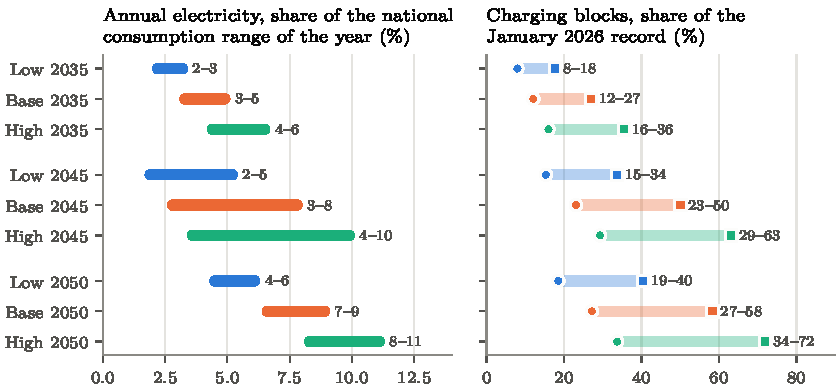
\includegraphics[width=\linewidth]{figures/fig4_materiality.pdf}
\caption{Materiality. Left: annual electricity as a share of the national consumption range of the year (2035: Fingrid Q3/2026 outlook, 110--162~TWh; 2045: Fingrid system vision 2023, 131--359~TWh; 2050: Long-term Climate Plan, final electricity consumption 134--180~TWh). Right: illustrative charging blocks as a share of the January 2026 record (circle: managed night block; square: concentrated evening block).}
\label{fig:materiality}
\end{figure}

\begin{table}[t]
\centering
\caption{Materiality against national references.}
\label{tab:materiality}
\small
\begin{tabular}{@{}llrrrrr@{}}
\toprule
Year & State & TWh & Share of national & Share of & Evening blocks, & Ratio to data- \\
 & & & range (\%) & 2025 use (\%) & \% of record & centre buildout (\%) \\
\midrule
2035 & Low & 3.5 & 2.2--3.2 & 4.2 & 8--18 & 6--14 \\
 & Base & 5.4 & 3.3--4.9 & 6.4 & 12--27 & 9--21 \\
 & High & 7.1 & 4.4--6.5 & 8.4 & 16--36 & 12--28 \\
\addlinespace
2045 & Low & 6.8 & 1.9--5.2 & 8.0 & 15--34 & 11--27 \\
 & Base & 10.2 & 2.8--7.8 & 12.0 & 23--50 & 16--40 \\
 & High & 12.9 & 3.6--9.9 & 15.3 & 29--63 & 21--51 \\
\addlinespace
2050 & Low & 8.2 & 4.5--6.1 & 9.7 & 19--40 & 13--32 \\
 & Base & 12.0 & 6.6--8.9 & 14.2 & 27--58 & 19--48 \\
 & High & 14.9 & 8.3--11.1 & 17.6 & 34--72 & 24--59 \\
\bottomrule
\end{tabular}

\sourcenote{National range: 110--162~TWh for 2035 \citep{fingrid2026prospects}; 131--359~TWh for 2045 \citep{fingrid2023vision}; 134--180~TWh final electricity consumption for 2050 \citep{meae2026ltcp}. 2025 use: 84.5~TWh \citep{fingrid2026q3}. Charging blocks: managed night block -- concentrated evening block, against 15,553~MW; they occur at different hours. Data-centre buildout: about 25~TWh (4.5~GW under construction) to 62~TWh (over 11~GW announced) \citep{merilehto2026blog}, at the 64\% utilisation implied by Fingrid's 28~TWh for nearly 5~GW of signed agreements \citep{fingrid2026prospects}.}
\end{table}

The comparison with data centres, which the 2030 study used to rank road transport, depends on which data-centre reference is used. Fingrid gives data-centre consumption of about 2~TWh in 2025, 9--18~TWh in 2030 and 11--35~TWh in 2035, and estimates that the projects with signed connection agreements by mid-August 2026, nearly 5~GW of nominal capacity, would use about 28~TWh if all were built \citep{fingrid2026prospects}, which implies an average utilisation of about 64\%. At that utilisation, the roughly 4.5~GW under construction corresponds to about 25~TWh a year and the more than 11~GW announced to about 62~TWh \citep{merilehto2026blog}. The author's base estimate for data-centre consumption in 2035 is over 30~TWh, above the signed-agreement figure and consistent with the further growth in agreements after mid-August. Against this capacity-based buildout range of 25--62~TWh, road transport is 6--28\% in 2035 and 13--59\% in 2050 (\cref{tab:materiality}); against the author's 30~TWh it is 12--24\% in 2035 and 27--50\% in 2050. The ministry's plan is the outlier: it puts data centres at 6.5~TWh in 2035 and just over 10~TWh in 2050 in three of its four scenarios, and at 14 and 30~TWh in the market-led one \citep{meae2026ltcp}. The lower figures are below the consumption implied by the capacity already under construction, so they understate data-centre demand rather than describe a plausible buildout. Taken at face value they would make road transport comparable to data centres in 2050. With data centres at 30~TWh in all four scenarios, the plan's 2050 totals would rise by roughly 20~TWh in the three lower scenarios to about 154--200~TWh, and road transport's share would fall to about 4--10\%. The volume hierarchy of the 2030 study therefore holds in 2050: road transport is secondary both to the national total and to a data-centre buildout consistent with the projects already under way.

The power side reads differently again. Average road-transport load in 2050, 0.9--1.7~GW, is 6--11\% of the 2026 record. The managed night block is 19--34\% of the record and the concentrated evening block 40--72\%. These ratios give scale only. The two blocks are charging levels in different hours, and without an hourly system profile neither is a contribution to the national peak; the night block falls in hours that normally have lower system load. What the comparison shows is that charging behaviour, not annual energy, decides whether road-transport charging runs near its 1--2~GW average or at 6--11~GW in winter evenings.

%=====================================================================
\section{Robustness}\label{sec:robust}
%=====================================================================
Every robustness variant re-solves $u$, so the 2025 statistic and the retained 2030 states remain exact; the script asserts both.

\subsection{One-way sensitivity}
\Cref{fig:tornado} shows the one-way sensitivity of the 2050 Base value. The two largest effects concern electricity per light-duty vehicle rather than adoption: 15\% lower use per EV by 2050, for example through efficiency gains or lower annual mileage, lowers 2050 to 10.5~TWh, and so does the calibration factor $\kappa$ converging to the engineering value of 1.0. A lower car ceiling of 85\% of entries, a plausible outcome of the softer 2035 rules combined with used imports, lowers 2050 by 0.7~TWh. The long-haul truck ceiling, fleet size and heavy-duty intensity each move the result by less than 0.5~TWh. Vehicle life and the PHEV tail matter little. The winter-day factor and the evening concentration do not change energy but move the 2050 concentrated evening block between 6.8 and 10.8~GW.

\begin{figure}[t]
\centering
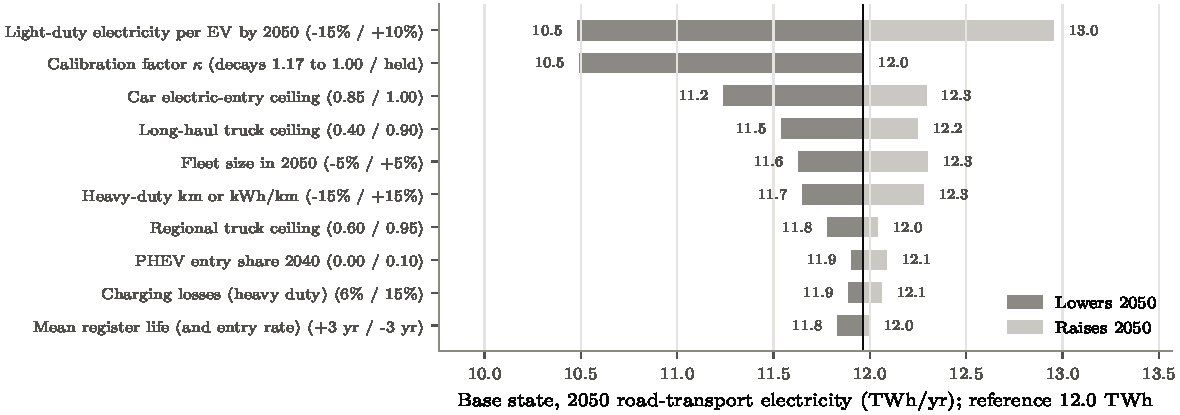
\includegraphics[width=\linewidth]{figures/fig5_tornado.pdf}
\caption{One-way sensitivity of 2050 Base road-transport electricity. Each variant re-anchors to the retained 2030 value.}
\label{fig:tornado}
\end{figure}

\subsection{Adoption delay and stalled adoption}
A genuine delay holds the 2030 entry shares for five or ten years and then follows the same curves that many years later, without renormalising to reach the same 2050 value. A five-year delay lowers 2050 by 9\% in Base and a ten-year delay by 19\% (\cref{tab:delay}, \cref{fig:delay}). Low is the most sensitive state (-14\% and -27\%) and High the least (-5\% and -11\%), because High is already near saturation by 2045. Stalled adoption, with entry shares frozen from 2030, lowers 2050 by 41\% in Low, 31\% in Base and 19\% in High. If entry shares had stayed at their 2025 values, electricity would reach 2.35~TWh in 2030 and 5.0~TWh in 2050. The difference between that path and the Base state, 7~TWh in 2050, is a measure of what the EU rules and the continued shift of the used-import market are assumed to deliver.

\begin{table}[t]
\centering
\caption{Delay and stalled adoption (TWh).}
\label{tab:delay}
\small
\begin{tabular}{@{}llrrrrr@{}}
\toprule
State & Variant & 2035 & 2040 & 2045 & 2050 & $\Delta$2050 \\
\midrule
Low & As constructed & 3.54 & 5.14 & 6.76 & 8.16 & -- \\
 & Delay 5 yr & 3.23 & 4.29 & 5.65 & 7.06 & $-14\%$ \\
 & Delay 10 yr & 3.23 & 3.98 & 4.80 & 5.95 & $-27\%$ \\
 & Stalled from 2030 & 3.23 & 3.98 & 4.49 & 4.79 & $-41\%$ \\
 & Stalled from 2035 & 3.54 & 4.87 & 5.85 & 6.53 & $-20\%$ \\
\addlinespace
Base & As constructed & 5.38 & 7.90 & 10.17 & 11.96 & -- \\
 & Delay 5 yr & 4.95 & 6.91 & 9.01 & 10.89 & $-9\%$ \\
 & Delay 10 yr & 4.95 & 6.48 & 8.02 & 9.72 & $-19\%$ \\
 & Stalled from 2030 & 4.95 & 6.48 & 7.59 & 8.30 & $-31\%$ \\
 & Stalled from 2035 & 5.38 & 7.64 & 9.34 & 10.52 & $-12\%$ \\
\addlinespace
High & As constructed & 7.11 & 10.28 & 12.93 & 14.86 & -- \\
 & Delay 5 yr & 6.77 & 9.47 & 12.02 & 14.08 & $-5\%$ \\
 & Delay 10 yr & 6.77 & 9.13 & 11.21 & 13.17 & $-11\%$ \\
 & Stalled from 2030 & 6.77 & 9.13 & 10.87 & 12.02 & $-19\%$ \\
 & Stalled from 2035 & 7.11 & 10.03 & 12.22 & 13.72 & $-8\%$ \\
\addlinespace
\multicolumn{2}{@{}l}{2025 entry shares frozen (2030: 2.35 TWh)} & 3.37 & 4.14 & 4.66 & 4.96 & $-59\%$ \\
\bottomrule
\end{tabular}

\sourcenote{Delay: 2030 entry shares held for $d$ years, then the original curves shifted by $d$ years. Stalled: entry shares frozen from the stated year. All variants retain the 2030 values; the last row does not.}
\end{table}

\begin{figure}[t]
\centering
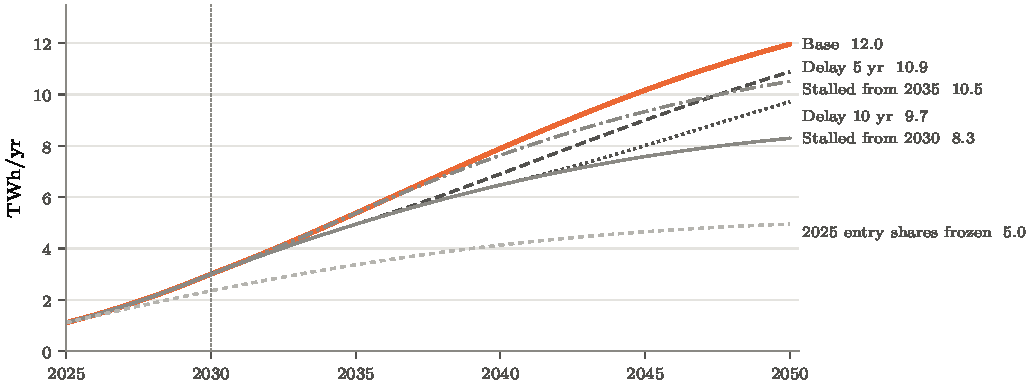
\includegraphics[width=\linewidth]{figures/fig6_delay_stall.pdf}
\caption{Delay and stalled-adoption variants of the Base state (TWh/yr).}
\label{fig:delay}
\end{figure}

\subsection{Charging behaviour and rebound}
The charging-behaviour stress (\cref{tab:loads} and \texttt{data/charging\_stress.csv}) spans managed charging to an extreme case of 85\% of light-duty energy in two hours. In the 2050 Base state the blocks run from 4.2~GW (managed, at night) through 5.4~GW (moderate evening) and 9.1~GW (concentrated evening) to 15.6~GW (extreme evening), the last equal to the 2026 record. A cold snap with winter-day energy 40\% above the annual mean lifts the concentrated evening block to 10.1~GW.

Managed charging creates its own risk when it is interrupted. \Cref{tab:rebound} curtails the managed light-duty night load (3.4~GW in Base, 4.1~GW in High) for two or four hours in 2050 and recovers half or all of the withheld energy afterwards, within the charging power that is plugged in. Two equipment assumptions bracket the result: 30\% of electric vehicles plugged in at 7.4~kW, or 50\% at 11~kW. With the first, the headroom above the managed load is only 1.9~GW in Base and 1.7~GW in High. Recovering all the energy withheld in a four-hour curtailment then takes at least 7.1 hours in Base and 9.9 hours in High; within four hours, 5.9 and 9.8~GWh would still be missing, and curtailment plus recovery would not fit within the ten-hour night window. These cases are infeasible as overnight events: vehicles would depart short of charge or recovery would run into the morning. With the second assumption, headroom is about 10~GW, recovery takes less than two hours, and a synchronised restart, every plugged-in vehicle resuming at full power when a price or control signal clears, lifts light-duty charging to 6.8--13.1~GW in Base, above the concentrated evening light-duty block of 7.9~GW. The better equipped the fleet, the more important a staggered restart becomes; the weaker the equipment, the less curtailment a night can absorb.

\begin{table}[t]
\centering
\caption{Rebound after curtailment of managed light-duty night charging, 2050.}
\label{tab:rebound}
\scriptsize
\resizebox{\linewidth}{!}{\begin{tabular}{@{}lcccrrrrcr@{}}
\toprule
State & Plugged-in & Curtailed & Recovered & Head- & To recover & Min.\ time & Unrecovered & Fits & Synchronised \\
 & share, kW & (h) & fraction & room (MW) & (MWh) & (h) & after 4 h (MWh) & 10 h? & peak (MW) \\
\midrule
Base & 0.3, 7.4 & 2 & 0.5 & 1,916 & 3,383 & 1.8 & 0 & yes & 5,299 \\
Base & 0.3, 7.4 & 2 & 1 & 1,916 & 6,766 & 3.5 & 0 & yes & 5,299 \\
Base & 0.3, 7.4 & 4 & 0.5 & 1,916 & 6,766 & 3.5 & 0 & yes & 5,299 \\
Base & 0.3, 7.4 & 4 & 1 & 1,916 & 13,531 & 7.1 & 5,867 & no & 5,299 \\
Base & 0.5, 11 & 2 & 0.5 & 9,745 & 3,383 & 0.3 & 0 & yes & 6,766 \\
Base & 0.5, 11 & 2 & 1 & 9,745 & 6,766 & 0.7 & 0 & yes & 10,148 \\
Base & 0.5, 11 & 4 & 0.5 & 9,745 & 6,766 & 0.7 & 0 & yes & 10,148 \\
Base & 0.5, 11 & 4 & 1 & 9,745 & 13,531 & 1.4 & 0 & yes & 13,128 \\
High & 0.3, 7.4 & 2 & 0.5 & 1,658 & 4,098 & 2.5 & 0 & yes & 5,756 \\
High & 0.3, 7.4 & 2 & 1 & 1,658 & 8,197 & 4.9 & 1,565 & yes & 5,756 \\
High & 0.3, 7.4 & 4 & 0.5 & 1,658 & 8,197 & 4.9 & 1,565 & yes & 5,756 \\
High & 0.3, 7.4 & 4 & 1 & 1,658 & 16,393 & 9.9 & 9,762 & no & 5,756 \\
High & 0.5, 11 & 2 & 0.5 & 10,162 & 4,098 & 0.4 & 0 & yes & 8,197 \\
High & 0.5, 11 & 2 & 1 & 10,162 & 8,197 & 0.8 & 0 & yes & 12,295 \\
High & 0.5, 11 & 4 & 0.5 & 10,162 & 8,197 & 0.8 & 0 & yes & 12,295 \\
High & 0.5, 11 & 4 & 1 & 10,162 & 16,393 & 1.6 & 0 & yes & 14,261 \\
\bottomrule
\end{tabular}
}
\sourcenote{Available power = plugged-in share $\times$ charger power $\times$ (BEV cars + vans + half of PHEVs); headroom = available power minus the managed load. Min.\ time: recovered energy divided by headroom. Fits 10~h: curtailment plus minimum recovery time within the ten-hour night window. Synchronised peak: managed load plus all recovered energy in the first hour, capped at available power.}
\end{table}

\subsection{Top-down checks}
Four top-down checks bound the bottom-up result. First, fully electrifying the 2025 road vehicle-km at the engineering intensities would use 14.0~TWh, or 15.6~TWh with the light-duty calibration factor; the 2050 states use 52\%, 77\% and 95\% of the calibrated ceiling. Second, Statnett estimated that electrifying Norway's 2.7 million cars, at 12,000~km and 0.2~kWh/km, would use about 6.5~TWh, and vans, trucks and buses about 5~TWh more \citep{statnett2019}. Applying the same per-km intensity to Finland's 39.0 billion car-km gives 7.8~TWh for cars alone; the Base state's 8.3~TWh for 2.09 million BEVs is higher because it carries the 2025 statistical calibration and $u$. Third, Fingrid's own transport figures (\cref{tab:boundary}), less rail, lie just above the High state in 2035 and between Base and High in 2040. Fourth, the ministry's 11--15~TWh for all transport in 2050 brackets the Base state plus rail. None of the checks suggests that road transport could approach 20~TWh in Finland without a much larger fleet or substantially higher mileage.

%=====================================================================
\section{Implications for the power market and grids}\label{sec:implications}
%=====================================================================
\textbf{Flexibility is where road transport matters most.} Finnish demand growth is led by data centres, which are unlikely to flex much, so flexibility must come from other actors \citep{merilehto2026blog}. Fingrid notes that not all new electrification load can flex \citep{fingrid2026q3}, and electric boilers and batteries have limits \citep{merilehto2026blog}. The illustrative evening and night charging blocks differ by 1.0--1.7~GW in 2030 and 3.4--5.9~GW in 2050. How much charging could actually be shifted between hours, and what that would be worth for system adequacy, needs an hourly model that this paper does not provide. Charging is distributed and already metered, but its energy must be delivered by a deadline, which suits shifting within a night rather than covering multi-day scarcity.

\textbf{For distribution system operators}, the 2030 study's priorities carry forward with more weight: hosting-capacity monitoring, capacity-based tariffs, connection rules for high-power home charging and automated off-peak defaults. The rebound result adds two design requirements: staggered or randomised restart for any price or control signal that switches many chargers at once, which is also the regional peak risk that Finnish distribution research has flagged \citep{lut2026charging}, and limits on how long managed charging can be curtailed in a night when charging equipment is weak.

\textbf{For retailers, balancing parties and aggregators}, the value of EV charging lies in timing, controllability and aggregation, as in 2030, but at a larger scale. A fleet of two million BEVs that charges on spot prices behaves as a large, price-elastic but synchronised demand block. Reserve products such as FCR-D are already accessible to charging networks \citep{virta2026fcrd}. Bidirectional charging would widen the span further, but its scale before the mid-2030s depends on vehicle and charger availability that is not yet in place \citep{vattenfall2026v2g,ey2025flex}.

\textbf{For transmission and corridor planning}, road transport is not a reason to change the national energy balance, and it stays well below the data-centre buildout already under way, but both compete for connection capacity. Heavy-vehicle corridor charging is a new class of connection: a national peak of 75--354~MW by 2050, spread over highway sites whose number and size depend on coverage rules and traffic, mostly outside today's load centres and with little scope to flex.

%=====================================================================
\section{Limitations}
%=====================================================================
The 2025 value is preliminary and Statistics Finland does not publish how road-transport electricity is estimated; the calibration factor $\kappa$ absorbs that uncertainty and is tested. The age-mileage profile, the truck segmentation and the long-haul intensity are assumptions. Fleet sizes are held constant; the robustness test of $\pm5\%$ does not cover structural change in car ownership or vehicle-km, such as automation or a modal shift. The charging blocks are stylised; no hourly system profile, diversity, distribution-network topology or price is modelled, so the paper makes no claim about the change in national peak or adequacy. Hydrogen trucks, rail electrification and e-fuels are outside the boundary. Policy is represented by entry-share ceilings rather than modelled compliance. The national comparisons use consumption ranges from different sources and definitions (total consumption for Fingrid, final consumption for the ministry), and the ministry's 2050 totals rest on data-centre assumptions below the capacity already under construction. The data-centre buildout range converts capacities to energy at a single utilisation and does not model commissioning timing. The scenarios are assumed planning states; they assign no probabilities.

%=====================================================================
\section{Conclusion}
%=====================================================================
Extended to 2050, the central conclusion of the 2030 study survives. Road-transport electrification in Finland grows from 1.1~TWh in 2025 to 8--15~TWh in 2050. That is 4.5--11\% of national final electricity consumption in the Long-term Climate Plan's 2050 scenarios, so road transport remains a secondary national energy-volume driver. It is also well below data centres if their buildout follows the projects already under construction and announced, at roughly 25--62~TWh a year; only the ministry's low data-centre assumption of just over 10~TWh would make the two comparable. Its power footprint matters more. An illustrative winter-evening charging block of 6--11~GW in 2050, against a 15.6~GW record, compares with a managed night block of 3--5~GW. Whether managed charging becomes a flexibility asset or a rebound risk depends on tariffs, automation, charging equipment and how control signals are staggered. Heavy vehicles add a smaller energy volume but a distinct depot and corridor connection problem. The variables to track are therefore the number of electric vehicles, but also the share of charging that is managed, the electricity used per vehicle, and the pace at which megawatt-scale depots and corridor sites are connected.

\FloatBarrier
\appendix
\section{Reproduction of the 2030 study}
\begin{table}[h]
\centering
\caption{Reproduction of the 2030 study's published numbers from its stated inputs.}
\label{tab:reproduction}
\small
\begin{tabular}{@{}lrr@{}}
\toprule
Quantity in the 2030 study & Reproduced & Published \\
\midrule
2030 low (GWh), 1112$\times$(1+0.15)\^{}5 & 2,236.63 & 2237 \\
2030 base (GWh), 1112$\times$(1+0.22)\^{}5 & 3,005.41 & 3005 \\
2030 high (GWh), 1112$\times$(1+0.28)\^{}5 & 3,820.80 & 3821 \\
2030 low (TWh, abstract) & 2.24 & 2.24 \\
2030 high (TWh, abstract) & 3.82 & 3.82 \\
2030 base (TWh, abstract 'about 3.0') & 3.01 & 3 \\
CAGR 2014-2024 (\%) & 74.31 & 74.3 \\
CAGR 2016-2025 (\%) & 68.79 & 68.8 \\
CAGR 2019-2024 (\%) & 60.48 & 60.5 \\
CAGR 2020-2025 (\%) & 54.58 & 54.6 \\
CAGR 2022-2025 (\%) & 52.59 & 52.6 \\
CAGR 2023-2025 (\%) & 42.58 & 42.6 \\
2025 share of 84.6 TWh (\%) & 1.31 & 1.31 \\
2025 average load (MW) & 126.94 & 127 \\
2030 base average load (MW) & 343.08 & 343 \\
2030 base daily energy (GWh) & 8.23 & 8.2 \\
2030 evening block 70\%/3 h (GW) & 1.92 & 1.92 \\
2030 managed block 100\%/10 h (GW) & 0.82 & 0.8 \\
2025-2030 base increment (TWh) & 1.89 & 1.9 \\
Table 4 bottom-up total (TWh) & 3.00 & 3 \\
Table 6 row 1 (MW) & 300.00 & 300 \\
Table 6 row 2 (MW) & 750.00 & 750 \\
Table 6 row 3 (MW) & 1,250.00 & 1250 \\
\bottomrule
\end{tabular}

\sourcenote{The 14 annual values of the 2012--2025 series (Appendix C of the 2030 study) are also asserted individually. Run \texttt{python model/model.py}.}
\end{table}

\section{Data cut-off and reproducibility}
Public sources were reviewed through 8 November 2026. Statistics Finland tables 12sz, 11ie and 12jx were extracted from PX-Web on 8 November 2026. Announced plans, legislative proposals and project capacities are treated as stated, not as outcomes. The model uses only the Python standard library; figures use matplotlib. The 2030 study's CSV is held unchanged in \texttt{data/inputs/}, and the model verifies its checksum. The inputs, scripts, annual paths and robustness outputs accompany the article at \url{https://github.com/juhanimerilehto/road-electrification-2050-fi/tree/v1.0.0}.

\bibliographystyle{plainnat}
\bibliography{references}

\end{document}
